\chapter{Opis projektnog zadatka}
		
Cilj projekta jest razviti aplikaciju za olakšavanje koordinacije i praćenja životinja u divljini. Aplikacija omogućuje korisnicima da se prijavljuju i time sudjeluju u različitim akcijama. Aplikacija se dijeli na nekoliko ključnih dijelova:\\

\begin{packed_item}
\item[1)]Registracija. Ideja je da se neregistrirani korisnik može prijaviti te poslati zahtjev za registraciju sa željenom ulogom (istraživači, voditelji postaja, tragači) pružajući potrebne informacije:

\begin{packed_item}
	\item[a)] Korisničko ime
	\item[b)] Fotografija
	\item[c)] Lozinka 
	\item[d)] Postaja 
	\item[e)] Ime 
	\item[f)] Prezime 
	\item[g)] Email adresa
	
\end{packed_item}

%unos slike
		\begin{figure}[H]
			
\includegraphics[scale=0.4]{slike/login_screen.PNG} %veličina slike u odnosu na originalnu datoteku i pozicija slike
			\centering
			\caption{Primjer login screena (1)}
			\label{fig:promjene}
		\end{figure}
		
		%unos slike
		\begin{figure}[H]
			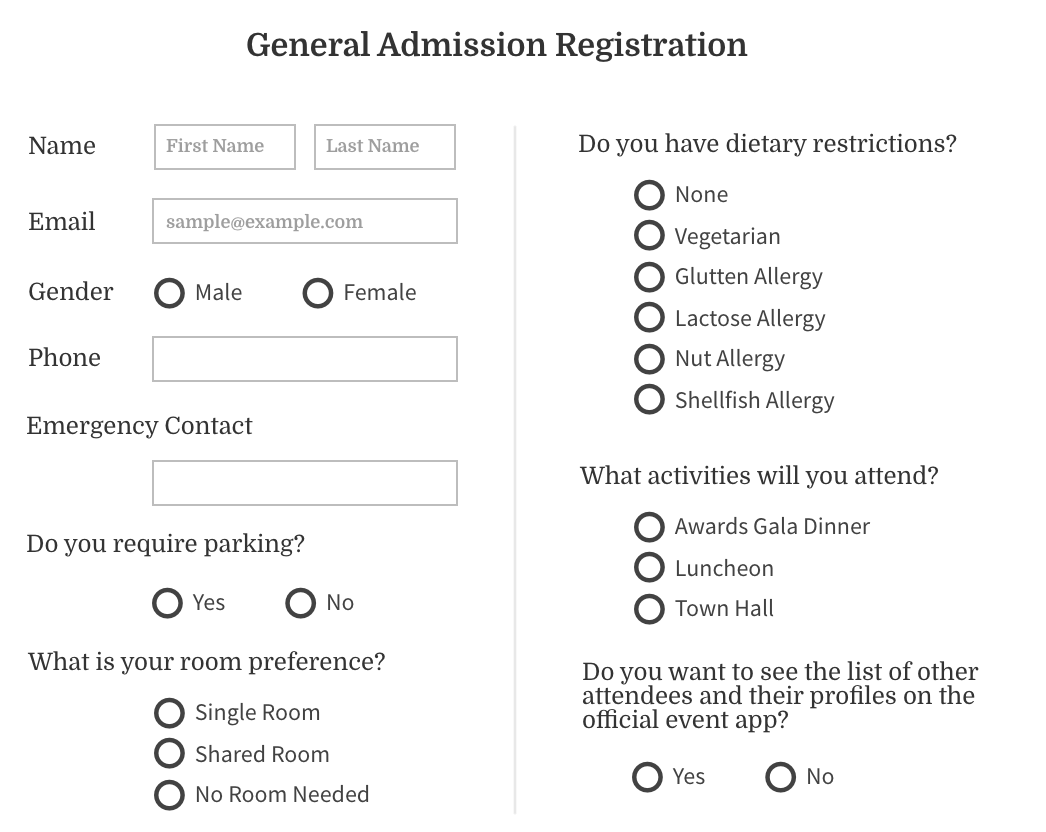
\includegraphics[scale=0.2]{slike/login_screen2.PNG} %veličina slike u odnosu na originalnu datoteku i pozicija slike
			\centering
			\caption{Primjer login screena (2)}
			\label{fig:promjene}
		\end{figure}
		
		%unos slike
		\begin{figure}[H]
			
\includegraphics[scale=0.9]{slike/biranje_uloge.PNG} %veličina slike u odnosu na originalnu datoteku i pozicija slike
			\centering
			\caption{Primjer biranja uloge}
			\label{fig:promjene}
		\end{figure}


Registracija završava potvrdom preko maila.\\

\item[2)] Administracija. \underline{Administrator} može vidjeti i upravljati podatcima korisnika. Ima mogućnost mijenjanja dodijeljenih prava i uloga te osobnih podataka. Nakon što se korisnik registrira, potrebna je dodatna potvrda od strane administratora za \underline{istraživače} i \underline{voditelje}.\\


\item[3)] Definiranje postaja. \underline{Voditelj} definira svoje postaje (npr postaja Lonjsko Polje) te bira \underline{tragače} koji su dio njihove postaje i koji su osposobljeni za pretraživanje. \\

\item[4)] Metode pretraživanja. Svaki \underline{tragač} treba imati sposobnost obavljanja pretrage:

\begin{packed_item}
	\item[a)] pješke
	\item[b)] dronom
	\item[c)] automobilom 
	\item[d)] cross motorom 
	\item[e)] brodom 
	\item[f)] helikopterom 
	
\end{packed_item}

Svaka metoda pruža različitu vidljivost i područje pokrivanja. Na primjer, zračno pretraživanje će obuhvatiti veće područje, ali neće pružiti toliko detalja kao što bi se dobilo pješačenjem.\\

\item[5)] Praćenje životinja. Praćene životinje na sebi imaju GPS uređaj koja našoj aplikaciji odašilje njegovu lokaciju. Podatci praćenih životinja:

\begin{packed_item}
	\item[a)] zadnje mjesto lokacije
	\item[b)] naziv vrste
	\item[c)] slika 
	\item[d)] opis 
	
\end{packed_item}

se zapisuju i pamte. Tragač može i ostaviti dodatni komentar.\\

\item[6)] Akcija pretraživanja. \underline{Istraživači} mogu započeti nove akcije pretraživanja i praćenja s detaljima određene vrste, jedinke ili staništa. Za svaku akciju imenuje se jedan istraživač koji surađuje s voditeljima postaja kako bi odabrao tragače s odgovarajućim kvalifikacijama za tu akciju. Na jednoj akciji mogu biti tragači različitih postaja. Istraživač uz pomoć karte zadaje tragačima zadatke. Zadatci mogu uključivati prelazak određene rute, stizanje do određene lokacije te postavljanje kamera ili uređaja za praćenje. Svaki zadatak može biti obogaćen dodatnim komentarom od strane istraživača. \underline{Tragač} se sam može maknuti iz akcije pri završetku zadanih zadataka. \\

%unos slike
		\begin{figure}[H]
			
\includegraphics[scale=0.5]{slike/pr_biranja_akcija.PNG} %veličina slike u odnosu na originalnu datoteku i pozicija slike
			\centering
			\caption{Primjer stranice za prihvaćanja/odbijanja akcija (1)}
			\label{fig:promjene}
		\end{figure}

%unos slike
		\begin{figure}[H]
			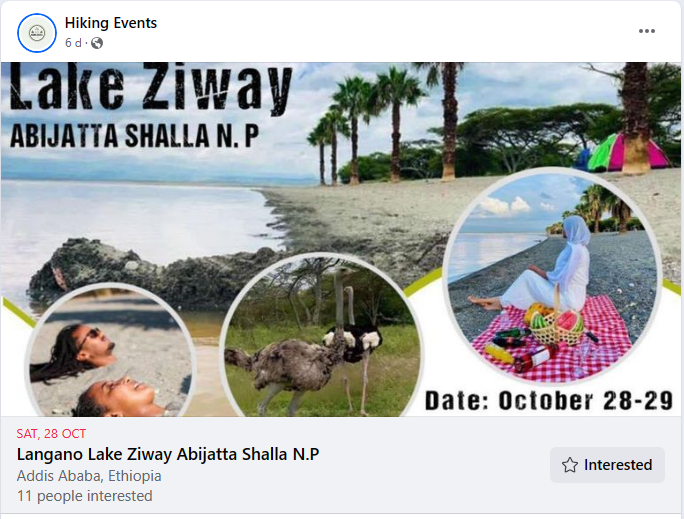
\includegraphics[scale=0.8]{slike/pr_biranja_akcija2.PNG} %veličina slike u odnosu na originalnu datoteku i pozicija slike
			\centering
			\caption{Primjer stranice za prihvaćanja/odbijanja akcija (2)}
			\label{fig:promjene}
		\end{figure}

\item[7)] Kartografski prikaz. Istraživaču će se informacije o pozicijama životinja, tragača i postaja pokazivati preko interaktivne karte. Istraživač ima opciju odabira između različitih opcija pri stvaranju karte:

\begin{packed_item}
	\item[a)] povijesne pozicije svih praćenih životinja, mogu se filtrirati po vrsti, ili pojedinačno
	\item[b)] povijesne pozicije svih praćenih životinja, mogu se filtrirati po vrsti, ili pojedinačno
	\item[c)] povijesne pozicije svih tragača na određenoj akciji te filtriranje prema vrsti prijevoza ili pojedinačno 
	\item[d)] trenutne pozicije svih tragača u toj akciji 
	
\end{packed_item}

Informacije u povijesnim podatcima se pokazuju u obliku toplinskih karata.
\underline{Tragaču} se na karti prikazuju trenutna lokacija svih ostalih tragača koji sudjeluju u akciji te trenutnu lokaciju praćenih životinja.
 Također, i tragači i istraživač mogu ostaviti komentare za ostale sudionike u akciji na karti.
 
 %unos slike
		\begin{figure}[H]
			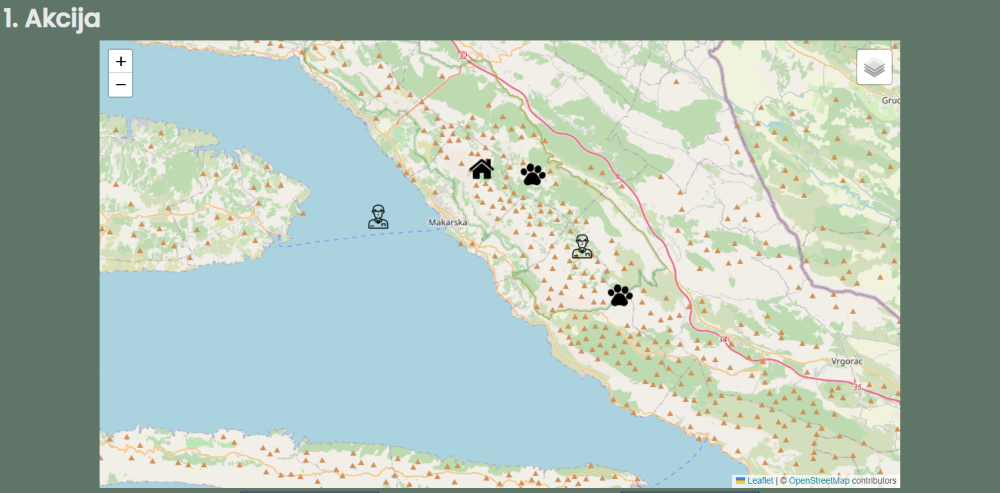
\includegraphics[scale=0.4]{slike/map_tracking.PNG} %veličina slike u odnosu na originalnu datoteku i pozicija slike
			\centering
			\caption{Primjer kartografskog prikaza (1)}
			\label{fig:promjene}
		\end{figure}


%unos slike
		\begin{figure}[H]
			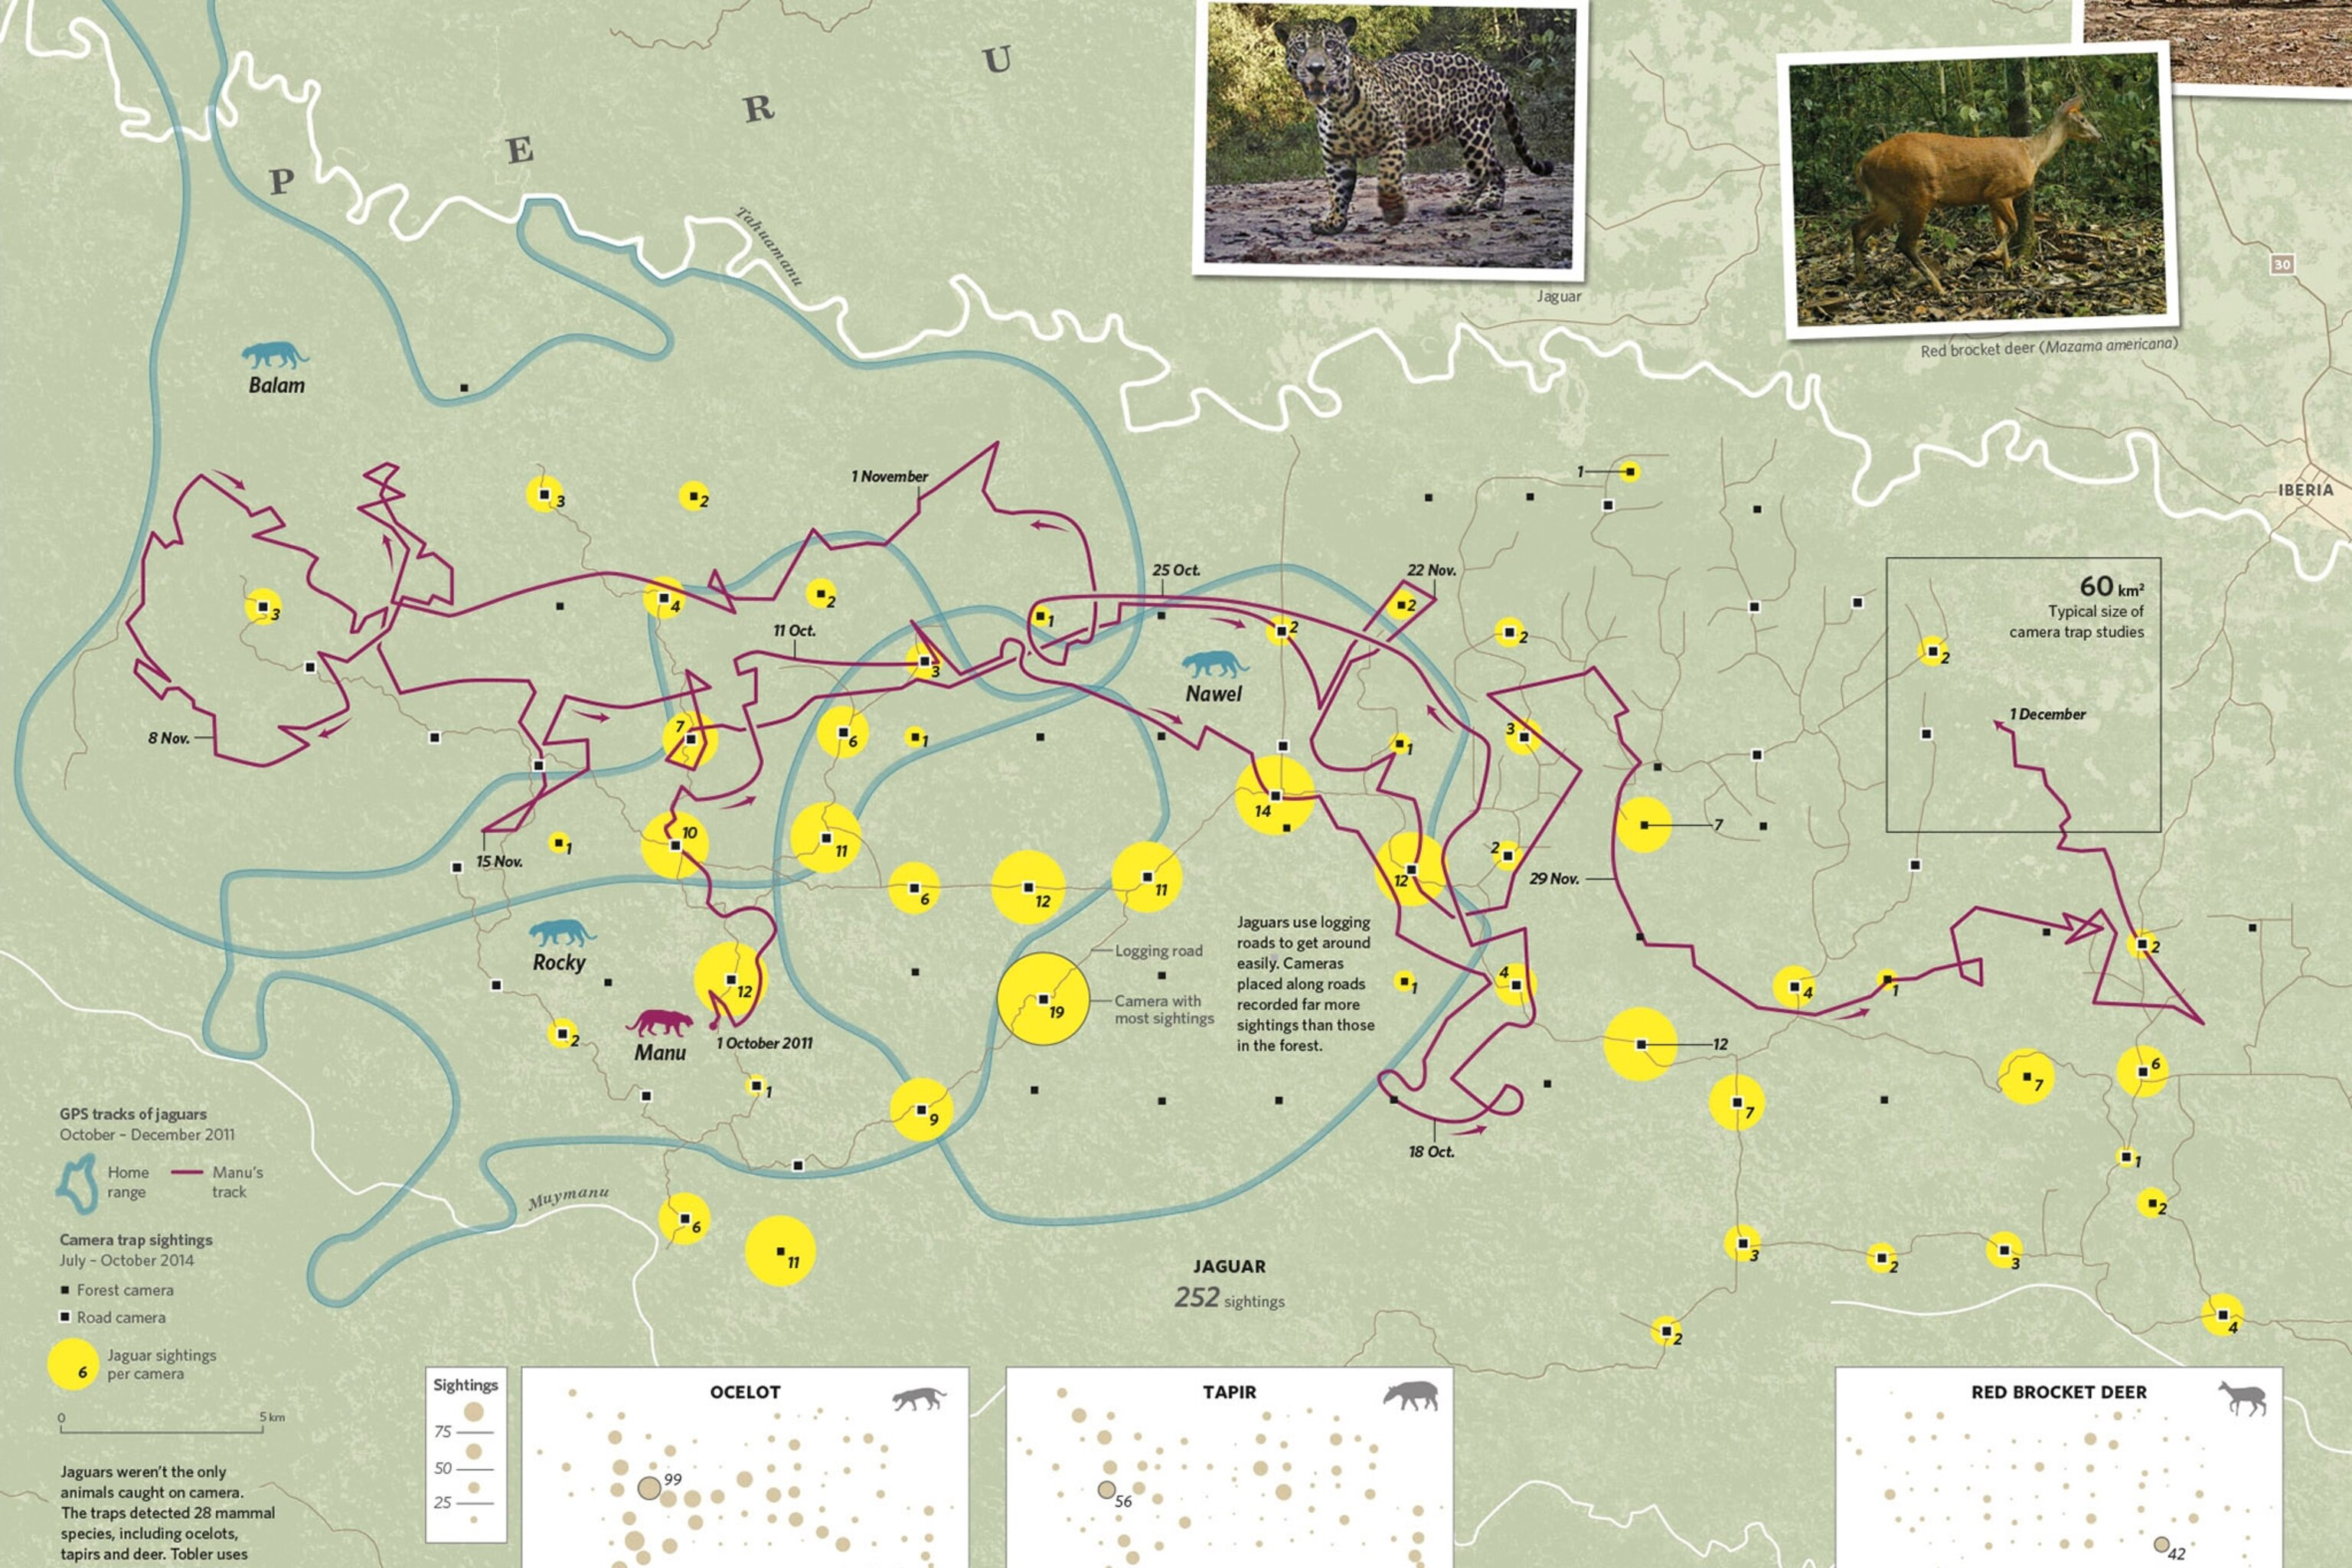
\includegraphics[scale=0.1]{slike/map_tracking2.PNG} %veličina slike u odnosu na originalnu datoteku i pozicija slike
			\centering
			\caption{Primjer kartografskog prikaza (2)}
			\label{fig:promjene}
		\end{figure}


\end{packed_item}



		